%%%% Proceedings format for most of ACM conferences (with the exceptions listed below) and all ICPS volumes.
\documentclass[sigconf]{acmart}
%%%% As of March 2017, [siggraph] is no longer used. Please use sigconf (above) for SIGGRAPH conferences.

%%%% Proceedings format for SIGPLAN conferences 
% \documentclass[sigplan, anonymous, review]{acmart}

%%%% Proceedings format for SIGCHI conferences
% \documentclass[sigchi, review]{acmart}

%%%% To use the SIGCHI extended abstract template, please visit
% https://www.overleaf.com/read/zzzfqvkmrfzn


\usepackage{booktabs} % For formal tables
\usepackage{amsmath} % For better math equations
\usepackage{amssymb} % For better math symbols
\usepackage{bbm} % For better math numerical symbols
\usepackage{amsthm} % For better theorem structures
\usepackage[ruled]{algorithm2e} % For algorithms
\usepackage{subcaption} % For multiple images in a section
\usepackage{natbib} % For better citations
\usepackage{cancel} % For better cancellations in equations

\renewcommand{\algorithmcfname}{ALGORITHM}

% Theorem section style and definition
\theoremstyle{plain}
\newtheorem{theorem}{Theorem}[section]

% Definition section style and definition
\theoremstyle{definition}
\newtheorem{definition}{Definition}[section]

% Copyright
% \setcopyright{none}
%\setcopyright{acmcopyright}
%\setcopyright{acmlicensed}
\setcopyright{rightsretained}
%\setcopyright{usgov}
%\setcopyright{usgovmixed}
%\setcopyright{cagov}
%\setcopyright{cagovmixed}


% DOI
% \acmDOI{10.475/123_4}

% ISBN
% \acmISBN{123-4567-24-567/08/06}

%Conference
\acmConference[CS 597 Spring'19 UIC]{UIC}{April 2019}{Chicago, Illinois USA}
\acmYear{2019}
\copyrightyear{2019}


\acmArticle{4}
\acmPrice{15.00}



\begin{document}
\title{Fairness of Envy-freeness in Maximum Nash Welfare of Specialized Markets}


\author{Shail Rakhunde}
\affiliation{%
  \institution{University of Illinois at Chicago}
  \city{Chicago}
  \state{Illinois}
}
\email{srakhu2@uic.edu}


\begin{abstract}
\label{section_abstract}

Maximum Nash welfare (MNW) solution to the resource allocation problem has garnered attention for satisfying an illusive combination of efficiency and fairness properties in the form of Pareto Optimality (PO) and approximated envy-freeness (EF1) for indivisible goods with additive valuations \cite{caragiannis2016unreasonable}. Though, individually, each of those properties are easily achievable by maximizing the utilitarian vs egalitarian parameters of a welfare solution, a combination of them brings in a rare feat for MNW solution. Most of the existing research in this area are based on the assumption that the goods showcase additive valuations. But the real-world is hardly defined as such and is full of examples showing non-additive valuations of various forms. We extend the resource allocation problem with two forms of non-additive utilities; complementary and substitute. We simulate the MNW solutions with such dependent valuations. The experimental analysis show that the MNW solution satisfies the relaxed version of envy-freeness property along with the efficiency.  We show that MNW solution is both Pareto optimal and envy-free up to $k$ goods (EFk), where $k$ represents a maximum external dependency of valuation of the good.

\end{abstract}

%
% The code below should be generated by the tool at
% http://dl.acm.org/ccs.cfm
% Please copy and paste the code instead of the example below.
%
\begin{CCSXML}
<ccs2012>
<concept>
<concept_id>10010405.10010455.10010460</concept_id>
<concept_desc>Applied computing~Economics</concept_desc>
<concept_significance>500</concept_significance>
</concept>
<concept>
<concept_id>10003752.10010070.10010099.10010101</concept_id>
<concept_desc>Theory of computation~Algorithmic mechanism design</concept_desc>
<concept_significance>300</concept_significance>
</concept>
</ccs2012>
\end{CCSXML}

\ccsdesc[500]{Applied computing~Economics}
\ccsdesc[300]{Theory of computation~Algorithmic mechanism design}

\keywords{Fair division, Resource allocation, Indivisibility, Nash social welfare, Envy-freeness}

\maketitle

\section{Introduction}

\begin{figure}
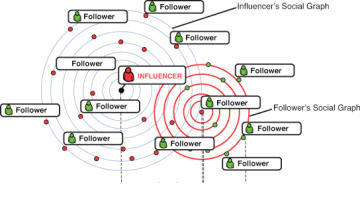
\includegraphics[width=2in]{images/influence_net.jpg}\Description{Sample Influence Network}
\caption{An example influence network with information flow diffusion}
\end{figure}

Influence and information flow is one of the important attributes of the graphs. Patterns emerge in any human interaction which extends to many academic disciplines such as psychology, sociology, economics, and anthropology. With the advent of social media, we now have a well documented, semistructured data at our disposal. As more and more people get access to Facebook, Twitter, YouTube, and the likes, it further necessitates the research in various multidisciplinary research communities. Traditionally, it's been extensively analyzed in the online recommendation and advertising. Recently, new complications have started to emerge in regards to the spread of news, fake news, hoax and their effects on society, government, nations and individuals.

Social influence has always been in attention because of the strong viral powers associated. With the emergence and wide usage of social media, it has achieved the scale it couldn't have without it. With billions of active users at any time, social media generates a tremendous amount of information about people, news, politics and social issues. This information is used by various groups to define and target their business operations such as marketing \cite{hoffman2010can}, campaigning \cite{cogburn2011networked, ratkiewicz2011detecting, shirky2011political, tumasjan2010predicting}, community profiling \cite{papadopoulos2012community, zhou2012community, chandrasekaran2013social} to specific user groups.

Many traditional machine learning methods have addressed the topic of network influence \cite{kempe2003maximizing, abebe2018opinion, albi2017opinion, acemoglu2011opinion, lawyer2015understanding, harada2015forecasting, islamdeepdiffuse}. Some of these methods try to model a specific concept from various disciplines of human studies. For example, \cite{matsubara2012rise} models the social influence dynamics from the "Susceptible-Infected" model where we label each node on its probability of getting influenced along with the current class association or infection. 

Node embedding has recently emerged as an effective and scalable tool for mining all kinds of networks. Existing research has produced excellent results on learning the structure, relationship, and spatial coexistence. DeepWalk \cite{perozzi2014deepwalk}, which we will describe below, learns the node representations in an embedded vector space. It is a scalable method, works on locality. Many tasks such as node classification, edge regeneration, continuity analysis are found to be outperforming traditional methods using the deep neural network based node embeddings.

But most of the current node embedding methods are restricted to a static analysis of networks \cite{chen2018tutorial, grover2016node2vec, tang2015line, perozzi2017don, tu2016max, cao2016deep, abu2017watch, cao2015grarep}. They take nodes and edges as input and learns the structure of the network. This is great for static networks and tasks based in that. But for tasks such as information propagation and diffusion, the model needs to understand the interaction between the nodes and should be able to encode that interaction in the same node embeddings.

To get node-level influence prediction, we introduce InfloWalk. Inspired by existing node embedding frameworks, InfloWalk tries to address the node influence information by training the node embedding algorithm on both network structure data as well as node influence data. We further experiment this node embedding method with 3 real-world dataset on the task of node classification. The results shows that the method outperforms the baselines.

Below we list the contributions of the paper:
\begin{enumerate}
\item A novel network embedding method which uses not only the network structure but also the influence and information flow networks. This successfully encodes the information flow in the network along with the network structure rather than just encoding the network structure like most of the existing embedding models.
\item The model is a simple extension of an existing network embedding framework. Because of the scalability and flexibility of the existing framework, this framework shows the same scalability and flex capabilities.
\item We test the framework on three real-world datasets to show the effectiveness of the proposed method.
\end{enumerate}



\section{Related Work and Preliminaries}
In this section, we will analyze the existing research in the related field and introduce some related concepts on which our framework is based on.

\subsection{Network Embeddings}
Network provides a universal way to structure various real-world information. It provides a way to represent any Entity-Relationship model with easy visualization. Each node has an associated set of features. For example, for social media, it can be a person with some gender, age, affiliations, etc. Similarly, each edge represents a type of relationship one node have with another. For example, a person may be a friend of another, another may be following a celebrity, etc. Nodes may form different networks on different attributes. For example, a friend circle, celebrity followers, related products network. Network studies involve identification of such node and edge features and studying the pattern in the structure of the graph. These studies can be categorized as local and global structures. With ever increasing social media user-base and diversity of the users, global structures are starting to make lesser sense in these types of networks. Our aim in this paper is to study the information flow and influence networks. These are inherently local to the network. This means we will start with one node of interest and try to learn its affiliations.

Network embedding can basically be seen as a mapping of each node in the network to a low dimensional latent representation. These low dimensional latent vectors can then be used in general network analysis tasks such as clustering, classification, labeling, link prediction, and visualizations. A few important features listed by \cite{chen2018tutorial} are adaptability, scalability, community awareness, low dimensions, and continuous vector space.

Traditionally, methods like Principle Component Analysis PCA \cite{krackhardt1988predicting} and Multi-dimensional Scaling (MDS) \cite{breiger1975algorithm} has widely been used to learn the low dimensional network representation. But many times traditional methods fail to identify local features as they see the network as a whole learning dataset at the same time. In the modern world of deep neural networks, we have new methods which try to solve these issues.

DeepWalk \cite{perozzi2014deepwalk} is one of the first such modern deep neural network based method. Highly inspired by the idea of word-embeddings, DeepWalk \cite{perozzi2014deepwalk} uses the same skip-gram model and applies it on random walks in the network. Both problems of generating walks and learning skip-gram models are extensively studied. They are parallelizable and hence highly scalable. DeepWalk \cite{perozzi2014deepwalk} introduces deep neural network methods to the world of graphs and networks.

DeepWalk \cite{perozzi2014deepwalk} works in three steps. First, creating a network representation in the form of a graph with nodes and edge lists. Second, it performs random walks on the network starting from any node and with a predefined walk-length. Third, these walks are passed to the skip-gram model which creates the node embeddings of a fixed low dimension for all the nodes in the network in an exact same fashion as word embeddings. The results outperform most of the traditional complex methods as you can see in the figure.

\begin{figure}
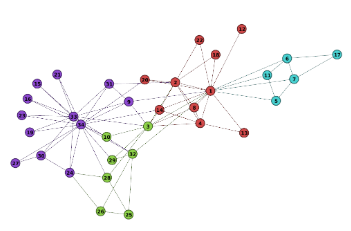
\includegraphics[width=2in]{images/karate_net.png}\Description{Karate Network}
\caption{The karate network}
\end{figure}

\begin{figure*}
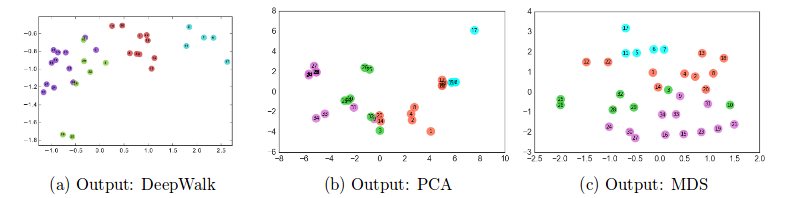
\includegraphics[width=7in]{images/karate_net_deepwalk.png}\Description{Karate Network Deepwalk}
\caption{Shows the results of classification using DeepWalk vs traditional methods on the karate network}
\end{figure*}

\subsection{Influence Network Learning}
Influence learning on a higher level can be defined as the effects of one node in the network on others. Influence is an intrinsic part of most of the networks found in real-world. Specifically, social media is completely dependent on the interaction between various users of the network. Any kind of interaction, be it in modern media or real-life, create influence. Influence can also be synonymous with information flow.

Traditionally, the influence was being modeled with a specialized domain-specific concept. For example, \cite{matsubara2012rise} defines social influence by modeling complex differential equations from an existing social model. A few other research uses behavior propagation modeling based on Ekman's model of emotion. \cite{wang2017gang} uses Guilt-by-association models which look into the features of the nodes in immediate neighborhood of the node under consideration. \cite{kempe2003maximizing} uses information diffusion mechanism to study the flow of information from source to across the network and further uses cascading to maximize the flow.

Influence network learning requires more data than just the nodes and the edges of the network. To model influence, we need information about every interaction between the nodes, for example, contents of the interaction, type of interaction, time of interaction, the response time, average response time, etc.

Most network embedding methods use and learn the network structure. But, they don't work on modeling the influence or the information flow. \cite{qiu2018deepinf} comes closest to the topic of this paper, where they use deep neural networks to predict the classification.

\hrule
x
\hrule

\section{Preliminaries}
In this section, we introduce the terminologies and theorems that have been used in further sections.

\subsection{Agents, Goods, Allocations, and Utilities}
Agents are a set of actors who try to claim the ownership over a set of goods. Goods are the set of objects which are to be allocated among the agents. Let us denote the set of $\mathit{n}$ agents with $\mathcal{N}$ and $\mathcal{M}$ be the set of $\mathit{m}$ indivisible goods.

Each agent have an associated utility for a particular good. In other words, each agent values a set of goods over others by a quantity. This is called a valuation function or an utility function. For agent $i$, the utility function is $f_i: M\mapsto \mathbb{R_+}$, where $\mathbb{R_+}$ is the set of positive real numbers. Here we assume each agent values the goods positively. We will encounter utility functions again in this section when we discuss some specific types of market later in the section.

An allocation is a distribution of goods into shares or portions. When we have only one quantity of each goods, each agent shows binary allocations. It owns/gets the good or it doesn't. It is illustrated in figure xyz1. If we have more than one count for any goods, an agent can get any permutation of it. We are assuming a single amount of each good unless specified otherwise. An allocation $\mathcal{A}_i\subseteq \mathcal{M}$ for any agent $i$.

For agent $i$, with an allocation $\mathcal{A}_i$ and its utility function for goods $f_i$, we can calculate the agent's total value of the allocation as
\begin{gather}
    F_i = \sum_{a \in \mathcal{A}_i} f_i(a)
\end{gather}

As mentioned previously, we will later see how this changes for different value functions.

\subsection{Additive goods and utilities}
Formally, additive goods/utilities are the ones who showcase mathematical additive properties. Additive goods are the ones whose utility is independent of others. Additive utilities are same as the one specified in previous section; that is, for agent $i$, the additive utility function is $u_i: M\mapsto \mathbb{R_+}$. Total utility of a set of goods/allocations is equal to the sum of all disjoint subsets.
\begin{gather}
    U_i = \sum_{a \in \mathcal{A}_i} u_{i,a}
\end{gather}

Where $\mathcal{A}_i$ is the allocation of goods to agent i and $u_{i,a}$ is agent i's utility for good a.

\subsection{Complementary goods and utilities}
Two goods are said to be complements if demand for one has some form of dependency over the demand of other. In other words, their demands are linked in such a way that increase in one raises the demand of the other, and same the decrease. A popular real-world example of complementary goods is razors blades. If the sell of razors increases, the demand for blades will rise too. This is an example of perfect complements. One can't use razors without blades or the other way. Real-world is full of such examples; burger and fries, hot dogs and buns, cars and gas, etc. Some of them are perfect complements, others are not.

In this paper, we define complements over pairs of adjacent goods. We denote complementing utilities for each agent i as: 

\begin{gather}
    v_i: \forall_{j < |M|/2} (M_{2j}, M_{2j+1})\mapsto \mathbb{R_+}
\end{gather}

An agent will earn the complementing utility if its allocation contains both the goods representing that value, otherwise not. If it does, it will be added to the additive utility to get the total utility of the allocation of agent i.

**How to write total utility in mathematical form?**

\subsection{Substituting goods and utilities}
/* Filler. Replace this

Two goods are said to be complements if demand for one has some form of dependency over the demand of other. In other words, their demands are linked in such a way that increase in one raises the demand of the other, and same the decrease. A popular real-world example of complementary goods is razors blades. If the sell of razors increases, the demand for blades will rise too. This is an example of perfect complements. One can't use razors without blades or the other way. Real-world is full of such examples; burger and fries, hot dogs and buns, cars and gas, etc. Some of them are perfect complements, others are not.

In this paper, we define complements over pairs of adjacent goods. We denote complementing utilities for each agent i as: 

\begin{gather}
    v_i: \forall_{j < |M|/2} (M_{2j}, M_{2j+1})\mapsto \mathbb{R_+}
\end{gather}

An agent will earn the complementing utility if its allocation contains both the goods representing that value, otherwise not. If it does, it will be added to the additive utility to get the total utility of the allocation of agent i.

*/

\subsection{Fairness, Envy, and Envy-freeness}
Fairness is one of the primary criteria in any resource allocation problem. The notion of fairness differs with the definition of the allocation problem. Consider the problem of division of a cake among $n$ people. Each person should receive $n$th part of the cake. We extend the problem by starting with $m$ cakes. Share of each person should now be $m/n$. The fairness criterion here is very loose as the only constraint we are trying to satisfy is equal distribution among all. In the same problem, we introduce the concept of age of a person. A person should receive a portion of a cake with respect to the age. Young ones will get more cake than the older. The fairness criteria now is to strictly get more cake if younger and not necessarily equal if same age. The criteria can further be varied if we introduce other types of food and preferences of people over these types.

One fairness criterion studied extensively in literature is Envy-freeness. Envy is defined as an amount with which an agent prefers an allocation of someone else. 

\subsubsection{Definition 3.1} Envy.
An agent $i$ with a value of $v_{ia}$ for a good $a$ which is allocated to agent $j$ who has a value of $v_{ja}$ for the same good $a$ envies agent $j$ by an
amount $e_{ij} = v_{ja} - v_{ia}$. The entity $e_{ij} \geq 0$ implies agent $i$ does not envy agent $j$, whereas $|e_{ij}|$ is the amount of envy $i$ has for $j$ otherwise. Extending the same to the entire allocation $\mathcal{A}_i$ instead of a single good, $E_{ij} = V_i(\mathcal{A}_j) - V_i(\mathcal{A}_i)$, where $V_i$ is the value function for agent $i$, and $\mathcal{A}_i$ and $\mathcal{A}_j$ are allocations of $i$ and $j$, respectively.

Envy-freeness (EF) is a notion of fair allocation where every agent prefers their own allocation over that of any other agent. In other words, every agent feels their allocation is better than or at least as valuable as the allocation of any other agent.

\subsubsection{Definition 3.2} Envy-freeness (EF).
An allocation is envy-free if $\mathcal{A}_i \succeq_i \mathcal{A}_j \forall i,j$ where $\mathcal{A}_i$ and $\mathcal{A}_j$ is the allocation of $i$ and $j$, respectively. Given a value function $V_i$ for agent $i$, $V_i(\mathcal{A}_i) \geq V_i(\mathcal{A}_j)$ $\forall i,j$. 

For a simple cake division problem, each person would want a piece of size greater than or at least equal to any other person. No one would want to exchange their piece with anyone else. This results in everyone having same sized pieces of the cake.

In the extended version of the problem, the idea of envy should reflect the age of the person. In an envy-free allocation, each person will have a piece of cake according to their own age and ensuring the fact that they don't want the piece of any other person. 

Fair distribution of a cake is an example of divisible goods. There always exist an envy-free solution for the allocation of divisible goods [cite]. Though, increasing the number of agents, increases the complexity of the envy-free allocation and it may take a very long time for computation [cite].

The problem gets difficult for indivisible goods. In a simple example with one item and two agents, where both have positive utilities for the item, the item can only be allocated to one of the agents. No matter which agent gets the item, the other agent will always envy for not getting the item. Envy-free division can not be guaranteed in general for the case of indivisible goods. The problem of determining whether an allocation exists, which is envy-free, is computationally hard [cite].

For feasibility, we weaken the constraint on envy-freeness and attempt allocation under these constraint.

\begin{definition}{Envy-free up to one good (EF1) \cite{caragiannis2016unreasonable}}
An allocation $\mathcal{A}$ is envy-free up to one good (EF1) if for all agents $i$, $j$, agent $i$ will stop envying agent $j$ if a good $g$, for some $g$ in $\mathcal{A}_j$ is dropped from the allocations of agent $j$, $\mathcal{A}_j$. Formally,
$$
    \forall i,j \in \mathcal{N}, \exists g \in \mathcal{A}_j, V_i(\mathcal{A}_i) \geq V_i(\mathcal{A}_j \backslash \{g\})
$$
\end{definition}

We further relax the envy-freeness fairness criterion for up to $k$ goods.

\begin{definition}{Envy-free up to $k$ goods (EFk).}
An allocation $\mathcal{A}$ is envy-free up to $k$ goods (EFk) if for all agents $i$, $j$, agent $i$ will stop envying agent $j$ if a set of goods $\mathcal{G} \subseteq \mathcal{A}_j$, such that $|\mathcal{G}| = k$, is dropped from the allocations of agent $j$, $\mathcal{A}_j$. Formally,
$$
    \forall i,j \in \mathcal{N}, k \leq |\mathcal{M}|, \exists \mathcal{G} \subseteq \mathcal{A}_j, || = k, V_i(\mathcal{A}_i) \geq V_i(\mathcal{A}_j \backslash \{\mathcal{G}\})
$$
\end{definition}

In other words, if agent $i$ doesn't envy agent $j$ once we drop some $k$ goods from agent $j$'s allocation $\mathcal{A}_j$, then the allocation is called envy-free up to $k$ goods (EFk).


\subsection{Welfare and Maximum Nash Welfare}
Welfare is a concept of an economic system which ensures happiness and well-being of all the participating agents with some agreed definition of happiness or well-being. It follows the idea of fairness from the previous section. A system which is fair to all the constituting members can be said to ensure the welfare of all the participants, and further, the welfare of the entire system. We adopt the terminology of welfare in the resource allocation problem. Given an allocation of goods among agents, we believe we have achieved welfare if we have a fair allocation for each agent.

Like fairness, the notion of welfare differs with the definition of the resource allocation problem. Following the example from the previous section, for the simple cake division problem, equal division of cake among all agents would achieve the welfare in cake distribution. In the extended version of the cake division problem, if each agent receives a fair amount of cake based on the fairness criterion of age, the division will ensure welfare of the system.

Three popular notions of welfare are often discussed in economics: utilitarian, egalitarian and Nash.

An utilitarian welfare strives to achieve maximum overall utility. In resource allocation problem, a good will be allocated to that agent who has the maximum value for it. This ensures the maximum possible usage of the goods. Here, the idea of fairness is specified as maximum utilization of the goods. In that sense, it provides the most efficient allocation. Utilitarian distribution does not ensure that each agent needs to receive some good. An agent who does not have the best value for any good, may not get any good. Also, it is possible that one may have best value for all of the goods and may end up receiving all the goods. In other words, utilitarian welfare, in trying to achieve the highest possible utility, does not ensure positive utility for all the participants.

An egalitarian welfare tries to maximize well-being or happiness of all agents. It strives to achieve equality of some type among all agents. In resource allocation problem, an egalitarian welfare system would not regard the utilities that agents have for various goods. A good should be allocated to an agent who owns the least amount. With a notion of equality defined, an egalitarian welfare provides the most fair allocation.

The simple cake division problem described above is both utilitarian and egalitarian. Every agent gets an equal share of the cake, and since every agent have the same value for the cake, the distribution achieves maximum efficiency. For the extended version of the cake division problem, the value for the cake is inversely proportional to the age of the person. The egalitarian welfare solution would allocate an equal amount of cake to everyone, whereas the utilitarian welfare solution would distribute cake based on the value.

The maximum Nash welfare (MNW) solution provides both fairness and efficiency. We follow the definition the MNW solution by Caragiannis, Ioannis, et al. \cite{caragiannis2016unreasonable}

\begin{definition}{Nash welfare (NW) or Nash product}
Nash welfare or Nash product is a product of utilities of agents for allocated goods

$$
    NW(\mathcal{A}) = \prod_{i \in \mathcal{N}} V_i(\mathcal{A}_i)
$$

for all agents $i$ in $\mathcal{N}$, where $V$ is the value function and $\mathcal{A}$ is the allocation.
\end{definition}

\begin{definition}{Maximum Nash welfare (MNW).}
MNW allocation is the one that maximizes the Nash welfare among all possible allocations

$$
    \mathcal{A}^{MNW} = \operatorname{arg\,max}_{A \in \prod_{|\mathcal{N}|}(\mathcal{M})} NW(\mathcal{A})
$$
\end{definition}


Maximum Nash welfare is widely known for its welfare guarantees. MNW is found to satisfy interesting properties in a fair allocation problem. MNW is efficient with satisfaction of the Pareto optimality, and it has an attractive fairness property in the form of envy-freeness.

Pareto optimal (PO) allocation is the one in which it is not possible to make allocations of one agent better without making another agent's allocation worse. Pareto efficiency specifies the impossibility of improvement for one agent without affecting other agents negatively. PO is used as a property of efficient allocations because an allocation will not be Pareto if one can find an alternate allocation which improves the welfare for at least one agent without hurting the welfare of any other agent. With existence of no such improvement, PO represents the best possible scenario under such efficiency preference criteria.

\begin{definition}{Pareto optimality (PO).}
An allocation $\mathcal{A}$ is Pareto optimal if no other allocation $\mathcal{A'}$ is feasible such that $V_i(\mathcal{A}_i') \geq V_i(\mathcal{A}_i)$ for all agents $i \in \mathcal{N}$ with $ V_j(\mathcal{A}_j') > V_j(\mathcal{A}_j)$ for some agent $j \neq i$ where, $V_i$ is the value function for any agent $i \in \mathcal{N}$.
\end{definition}

\begin{theorem}
Every MNW allocation is Pareto optimal (PO) over indivisible goods.
\end{theorem}

\begin{proof}
We follow a simple proof of Pareto optimality for MNW by Caragiannis, Ioannis, et al. \cite{caragiannis2016unreasonable}. It is trivial for every MNW allocation $\mathcal{A}$ to be PO because any alternate allocation $\mathcal{A}'$ that increases the utility of one agent without decreasing the utility of any other agent would result in increase in the Nash welfare of the alternate allocation $\mathcal{A}'$, that is $NW(\mathcal{A}') > NW(\mathcal{A})$, contradicting the assumption that the original MNW allocation $\mathcal{A}$ had the maximum/optimal NW of all the possible allocations. 
\end{proof}

Maximum Nash welfare allocation satisfy the elusive fairness property of envy-freeness (EF) defined in the previous section. This is further studied and proved in the next section.

With PO and EF, the maximum Nash welfare, in a great degree of simplicity, is one of the rare algorithms providing us with both efficiency and fairness standards. It is a good balance between the utilitarian vs. egalitarian trade-off. Also, attempting to maximize for utilitarian or egalitarian welfare conditions results in non-EF allocations \cite{caragiannis2016unreasonable}. In that sense, MNW allocation prevails over utilitarian and egalitarian allocation criteria for the strong PO and EF guarantees that it ensures.

\section{Experiments}
In this section, we describe the data, computations, and analysis of the features of the data.

We simulate the problem with $n = 2$ agents competing for allocation of $m$ goods where $m \in \{10, 8, 6, 4\}$. The goods are unrelated, and independent. Each agent has some utility for each of the goods. We generate $m$ additive utilities for each agent at random over $[0, 100)$ representing agent's value for $m$ goods. We further generate $m/2$ complementary utilities for each agent at random over $[0, 100)$ representing agent's valuation for pairs of goods. Each complementary utility represents the collective value an agent would get if both the goods are allocated to the agent. We generate 100 samples each with random seed [10, 20) for reproducibility. Overall, we have $1000$ such examples for each value of $m \in {10, 8, 6, 4}$. In addition to that, we map these examples on to four types of goods showing : i) Additive utilities ii) Complementing utilities iii) Substituting utilities type 1 iv) Substituting utilities type 2.  MNW is computed for each of these sample with respect to four types of utilities with algorithm 1.

\BlankLine

% Maximum Nash Welfare computation - value function abstracted
\begin{algorithm}
\caption{ Computing an MNW allocation }
\SetAlgoLined
\KwIn{ Agents $\mathcal{N}$, resources $\mathcal{M}$, value function $value\_f$, additive utilities $AU$, complementary/substituting utilities $CSU$ }
\KwOut{ An MNW allocation $ \mathcal{A}^{MNW}$ }
 $Max\_NW \leftarrow 0 $ \;
 $\mathcal{A}_{Max\_NW} \leftarrow \phi $ \;
 \For{all possible allocations $ \mathcal{A} (N \times M) $}{
  $NW_\mathcal{A} \leftarrow \prod_{i \in \mathcal{N}} value\_f(\mathcal{A}_i, AU, CSU) $ \;
  \If{$NW_{\mathcal{A}} > Max\_NW $}{
   $Max\_NW \leftarrow NW_{\mathcal{A}}$ \;
   $\mathcal{A}_{Max\_NW} \leftarrow \mathcal{A} $ \;
  }
 }
\end{algorithm}

% Nash Welfare/Product computation
% For additive, complementing, substituting (type 1 and 2) utilities
\begin{algorithm}
\caption{ Computing NW }
\SetAlgoLined

Pairwise Allocation: \\
$ PA = (\mathcal{A}) \rightarrow [min(\mathcal{A}_{i,2j}, \mathcal{A}_{i,2j+1}) \forall i \in \mathcal{N}, j < |\mathcal{M}|/2] $

\BlankLine

Substituting utilities - type 1: \\
$ SU_1 = (AU) \rightarrow [max(AU_{i,2j}, AU_{i,2j+1}) \forall i \in \mathcal{N}, j < |\mathcal{M}|/2] $

\BlankLine

Substituting utilities - type 2: \\
$ SU_2 = (AU) \rightarrow [(AU_{i,2j} + AU_{i,2j+1}) - rand(0, min(AU_{i,2j}, AU_{i,2j+1}))) \forall i \in \mathcal{N}, j < |\mathcal{M}|/2] $

\BlankLine
\BlankLine

$ NW_{additive} = (\mathcal{A}, AU) \rightarrow \mathcal{A} \cdot AU $

$ NW_{compl} = (\mathcal{A}, AU, CU) \rightarrow \mathcal{A} \cdot AU + PA(\mathcal{A}) \cdot CU $

$ NW_{subst1} = (\mathcal{A}, AU) \rightarrow \mathcal{A} \cdot (AU - PA(\mathcal{A})) + PA(\mathcal{A}) \cdot SU_1(AU) $

$ NW_{subst2} = (\mathcal{A}, AU) \rightarrow \mathcal{A} \cdot (AU - PA(\mathcal{A})) + PA(\mathcal{A}) \cdot SU_2(AU) $

\end{algorithm}

% Discussion on analysis of experiements starts here

% Percent EFness
\begin{figure}[h!]
  \centering
  \begin{subfigure}[b]{0.3\linewidth}
    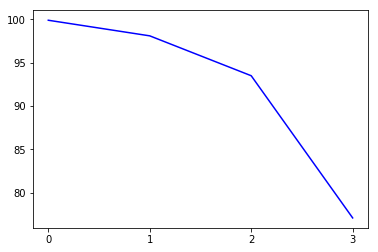
\includegraphics[width=\linewidth]{images/add/ef0_percent.png}
    \caption{}
  \end{subfigure}
  \begin{subfigure}[b]{0.3\linewidth}
    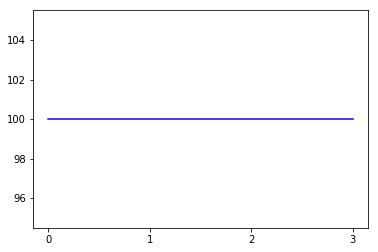
\includegraphics[width=\linewidth]{images/add/ef1_percent.png}
    \caption{}
  \end{subfigure}
  \begin{subfigure}[b]{0.3\linewidth}
    \includegraphics[width=\linewidth]{images/add/ef2_percent.png}
    \caption{}
  \end{subfigure}
  
  \begin{subfigure}[b]{0.3\linewidth}
    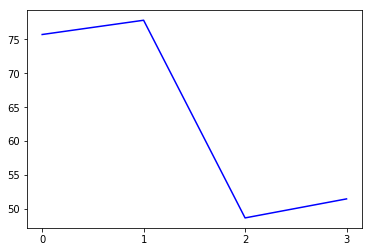
\includegraphics[width=\linewidth]{images/compl/ef0_percent.png}
    \caption{}
  \end{subfigure}
  \begin{subfigure}[b]{0.3\linewidth}
    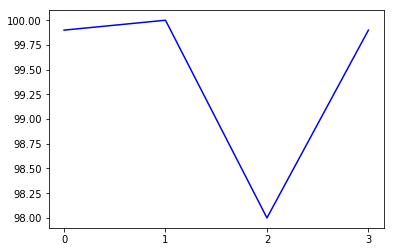
\includegraphics[width=\linewidth]{images/compl/ef1_percent.png}
    \caption{}
  \end{subfigure}
  \begin{subfigure}[b]{0.3\linewidth}
    \includegraphics[width=\linewidth]{images/compl/ef2_percent.png}
    \caption{}
  \end{subfigure}
    
  \begin{subfigure}[b]{0.3\linewidth}
    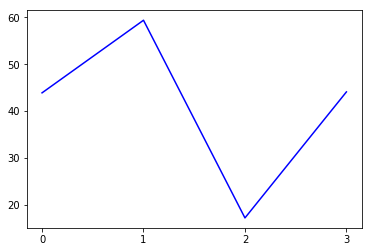
\includegraphics[width=\linewidth]{images/subst1/ef0_percent.png}
    \caption{}
  \end{subfigure}
  \begin{subfigure}[b]{0.3\linewidth}
    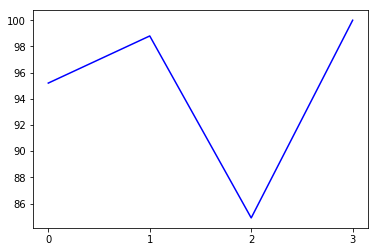
\includegraphics[width=\linewidth]{images/subst1/ef1_percent.png}
    \caption{}
  \end{subfigure}
  \begin{subfigure}[b]{0.3\linewidth}
    \includegraphics[width=\linewidth]{images/subst1/ef2_percent.png}
    \caption{}
  \end{subfigure}
    
  \begin{subfigure}[b]{0.3\linewidth}
    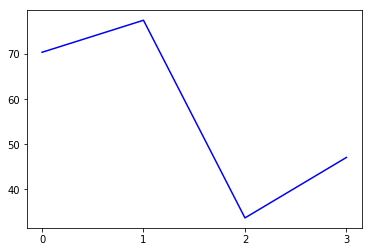
\includegraphics[width=\linewidth]{images/subst2/ef0_percent.png}
    \caption{}
  \end{subfigure}
  \begin{subfigure}[b]{0.3\linewidth}
    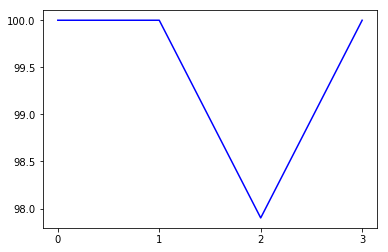
\includegraphics[width=\linewidth]{images/subst2/ef1_percent.png}
    \caption{}
  \end{subfigure}
  \begin{subfigure}[b]{0.3\linewidth}
    \includegraphics[width=\linewidth]{images/subst2/ef2_percent.png}
    \caption{}
  \end{subfigure}
  \caption{Percent EFk}
  \label{fig:efk}
  \small
    (a), (b), and (c) represent percent MNW allocations satisfying EF0, EF1, and EF2, respectively for additive utilities. (d), (e), (f), (g), (h), (i), (j), (k), and (l) represent that for complementing, substituting type-1, substituting type-2 utilities, respectively.
\end{figure}


Figure 4 shows the percent of samples which satisfies the envy-freeness specific criteria. Simple additive utilities gradually creates more envy with the decrease in number of goods as seen in Figure 4a. Figure 4a, 4b, and 4c collectively provides the experimental proof for envy-freeness up to one good (EF1) property of MNW allocations with additive valuations \cite{caragiannis2016unreasonable}. Figure 4f, 4i, and 4l, indicates pairwise complementary and substituting utilities follow envy-freeness up to 2 goods (EF2). Complementing and substituting utilities also showcase surprisingly high, if not perfect, EF1. In particular, substituting type-1 utilities for 4 goods and type-2 for 10, 8, and 4 goods have 100\% EF1.


% Mean Envy
\begin{figure}[h!]
  \centering
  \begin{subfigure}[b]{0.3\linewidth}
    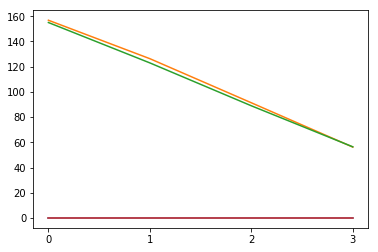
\includegraphics[width=\linewidth]{images/add/ef0_means.png}
    \caption{}
  \end{subfigure}
  \begin{subfigure}[b]{0.3\linewidth}
    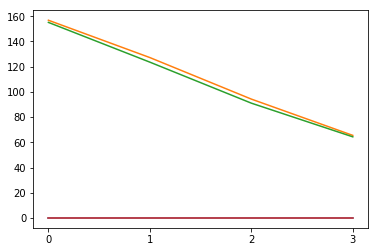
\includegraphics[width=\linewidth]{images/add/ef1_means.png}
    \caption{}
  \end{subfigure}
  \begin{subfigure}[b]{0.3\linewidth}
    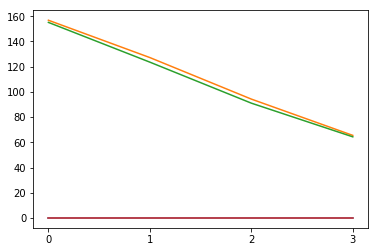
\includegraphics[width=\linewidth]{images/add/ef2_means.png}
    \caption{}
  \end{subfigure}
  
  \begin{subfigure}[b]{0.3\linewidth}
    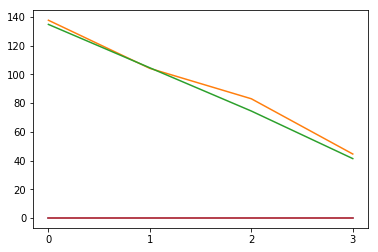
\includegraphics[width=\linewidth]{images/compl/ef0_means.png}
    \caption{}
  \end{subfigure}
  \begin{subfigure}[b]{0.3\linewidth}
    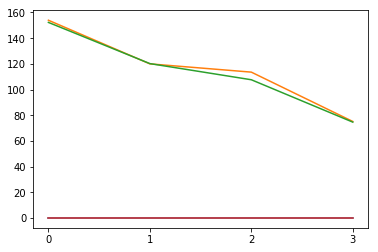
\includegraphics[width=\linewidth]{images/compl/ef1_means.png}
    \caption{}
  \end{subfigure}
  \begin{subfigure}[b]{0.3\linewidth}
    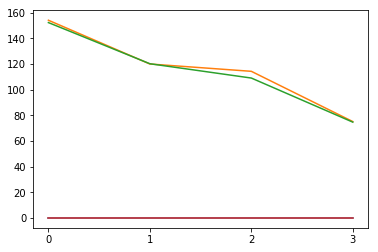
\includegraphics[width=\linewidth]{images/compl/ef2_means.png}
    \caption{}
  \end{subfigure}
    
  \begin{subfigure}[b]{0.3\linewidth}
    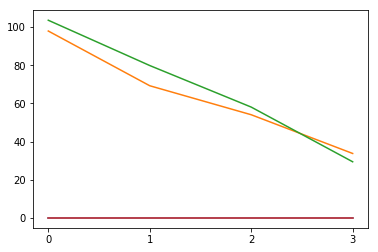
\includegraphics[width=\linewidth]{images/subst1/ef0_means.png}
    \caption{}
  \end{subfigure}
  \begin{subfigure}[b]{0.3\linewidth}
    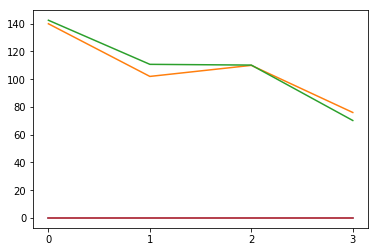
\includegraphics[width=\linewidth]{images/subst1/ef1_means.png}
    \caption{}
  \end{subfigure}
  \begin{subfigure}[b]{0.3\linewidth}
    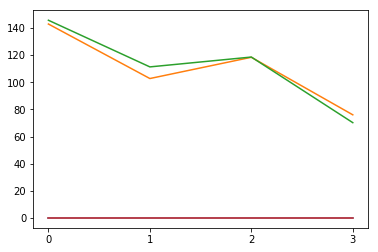
\includegraphics[width=\linewidth]{images/subst1/ef2_means.png}
    \caption{}
  \end{subfigure}
    
  \begin{subfigure}[b]{0.3\linewidth}
    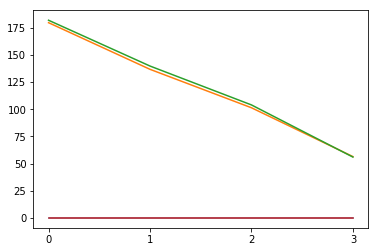
\includegraphics[width=\linewidth]{images/subst2/ef0_means.png}
    \caption{}
  \end{subfigure}
  \begin{subfigure}[b]{0.3\linewidth}
    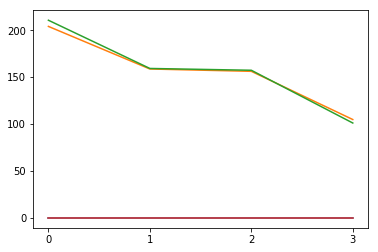
\includegraphics[width=\linewidth]{images/subst2/ef1_means.png}
    \caption{}
  \end{subfigure}
  \begin{subfigure}[b]{0.3\linewidth}
    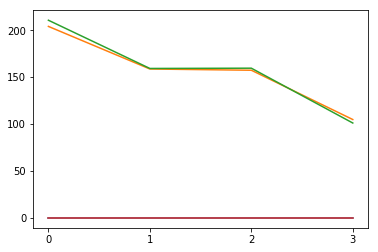
\includegraphics[width=\linewidth]{images/subst2/ef2_means.png}
    \caption{}
  \end{subfigure}
  \caption{Mean envy}
  \label{fig:efk}
  \small
    (a), (b), and (c) represent mean envy present in MNW allocations after dropping 0, 1, and 2 goods, respectively for additive utilities. (d), (e), (f), (g), (h), (i), (j), (k), and (l) represent that for complementing, substituting type-1, substituting type-2 utilities, respectively.
\end{figure}

% Mean Positive Envy
\begin{figure}[h!]
  \centering
  \begin{subfigure}[b]{0.3\linewidth}
    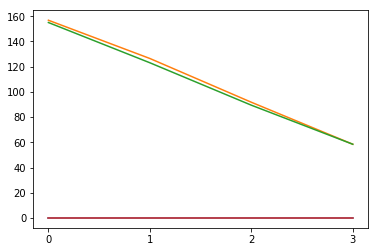
\includegraphics[width=\linewidth]{images/add/ef0_means_pos.png}
    \caption{}
  \end{subfigure}
  \begin{subfigure}[b]{0.3\linewidth}
    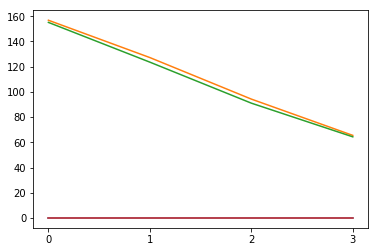
\includegraphics[width=\linewidth]{images/add/ef1_means_pos.png}
    \caption{}
  \end{subfigure}
  \begin{subfigure}[b]{0.3\linewidth}
    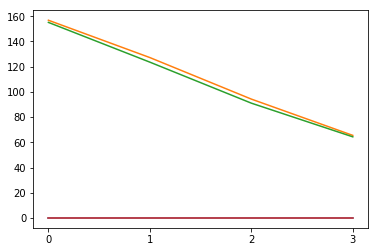
\includegraphics[width=\linewidth]{images/add/ef2_means_pos.png}
    \caption{}
  \end{subfigure}
  
  \begin{subfigure}[b]{0.3\linewidth}
    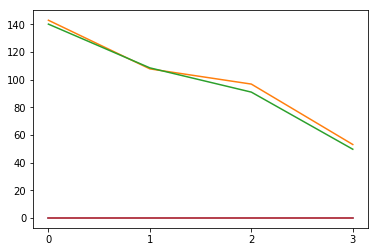
\includegraphics[width=\linewidth]{images/compl/ef0_means_pos.png}
    \caption{}
  \end{subfigure}
  \begin{subfigure}[b]{0.3\linewidth}
    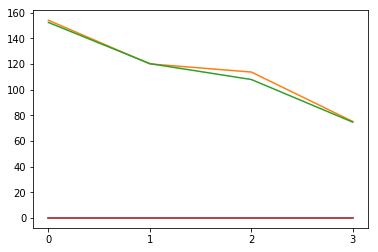
\includegraphics[width=\linewidth]{images/compl/ef1_means_pos.png}
    \caption{}
  \end{subfigure}
  \begin{subfigure}[b]{0.3\linewidth}
    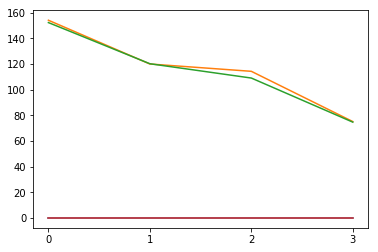
\includegraphics[width=\linewidth]{images/compl/ef2_means_pos.png}
    \caption{}
  \end{subfigure}
    
  \begin{subfigure}[b]{0.3\linewidth}
    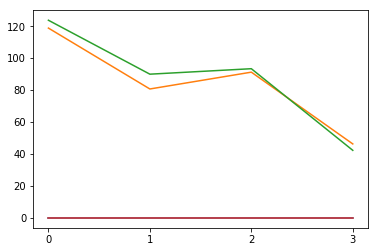
\includegraphics[width=\linewidth]{images/subst1/ef0_means_pos.png}
    \caption{}
  \end{subfigure}
  \begin{subfigure}[b]{0.3\linewidth}
    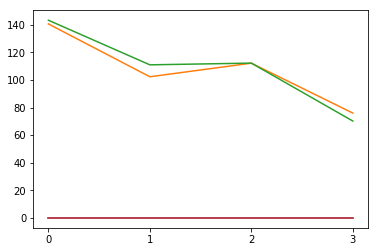
\includegraphics[width=\linewidth]{images/subst1/ef1_means_pos.png}
    \caption{}
  \end{subfigure}
  \begin{subfigure}[b]{0.3\linewidth}
    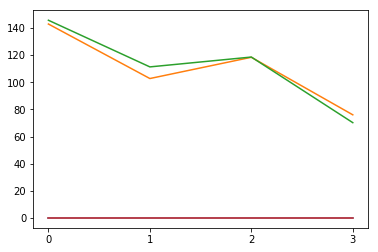
\includegraphics[width=\linewidth]{images/subst1/ef2_means_pos.png}
    \caption{}
  \end{subfigure}
    
  \begin{subfigure}[b]{0.3\linewidth}
    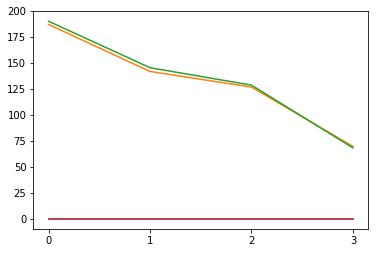
\includegraphics[width=\linewidth]{images/subst2/ef0_means_pos.png}
    \caption{}
  \end{subfigure}
  \begin{subfigure}[b]{0.3\linewidth}
    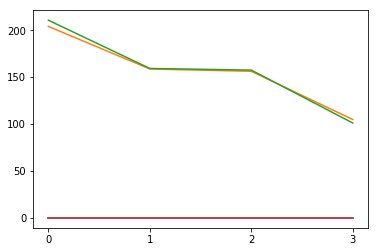
\includegraphics[width=\linewidth]{images/subst2/ef1_means_pos.png}
    \caption{}
  \end{subfigure}
  \begin{subfigure}[b]{0.3\linewidth}
    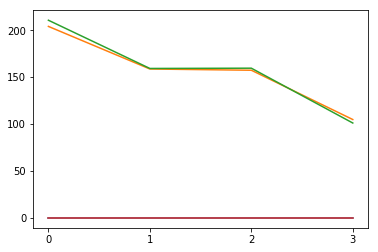
\includegraphics[width=\linewidth]{images/subst2/ef2_means_pos.png}
    \caption{}
  \end{subfigure}
  \caption{Mean positive envy}
  \label{fig:efk}
  \small
    (a), (b), and (c) represent mean positive envy (non-envy) present in MNW allocations after dropping 0, 1, and 2 goods, respectively for additive utilities. (d), (e), (f), (g), (h), (i), (j), (k), and (l) represent that for complementing, substituting type-1, substituting type-2 utilities, respectively.
\end{figure}

% Mean Negative Envy
\begin{figure}[h!]
  \centering
  \begin{subfigure}[b]{0.3\linewidth}
    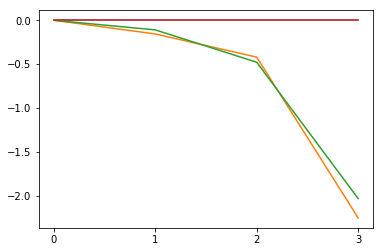
\includegraphics[width=\linewidth]{images/add/ef0_means_neg.png}
    \caption{}
  \end{subfigure}
  \begin{subfigure}[b]{0.3\linewidth}
    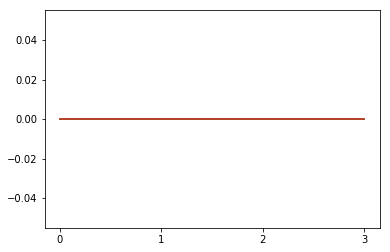
\includegraphics[width=\linewidth]{images/add/ef1_means_neg.png}
    \caption{}
  \end{subfigure}
  \begin{subfigure}[b]{0.3\linewidth}
    \includegraphics[width=\linewidth]{images/add/ef2_means_neg.png}
    \caption{}
  \end{subfigure}
  
  \begin{subfigure}[b]{0.3\linewidth}
    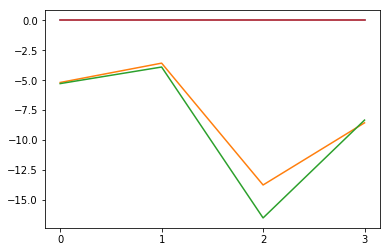
\includegraphics[width=\linewidth]{images/compl/ef0_means_neg.png}
    \caption{}
  \end{subfigure}
  \begin{subfigure}[b]{0.3\linewidth}
    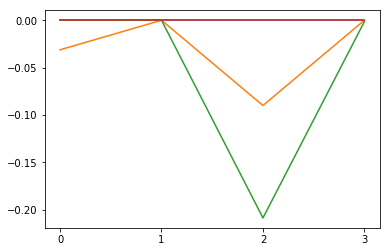
\includegraphics[width=\linewidth]{images/compl/ef1_means_neg.png}
    \caption{}
  \end{subfigure}
  \begin{subfigure}[b]{0.3\linewidth}
    \includegraphics[width=\linewidth]{images/compl/ef2_means_neg.png}
    \caption{}
  \end{subfigure}
    
  \begin{subfigure}[b]{0.3\linewidth}
    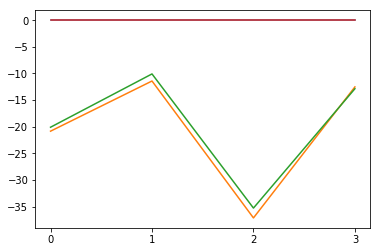
\includegraphics[width=\linewidth]{images/subst1/ef0_means_neg.png}
    \caption{}
  \end{subfigure}
  \begin{subfigure}[b]{0.3\linewidth}
    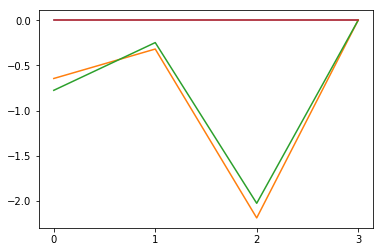
\includegraphics[width=\linewidth]{images/subst1/ef1_means_neg.png}
    \caption{}
  \end{subfigure}
  \begin{subfigure}[b]{0.3\linewidth}
    \includegraphics[width=\linewidth]{images/subst1/ef2_means_neg.png}
    \caption{}
  \end{subfigure}
    
  \begin{subfigure}[b]{0.3\linewidth}
    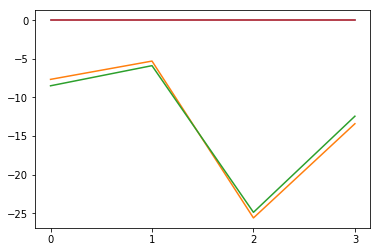
\includegraphics[width=\linewidth]{images/subst2/ef0_means_neg.png}
    \caption{}
  \end{subfigure}
  \begin{subfigure}[b]{0.3\linewidth}
    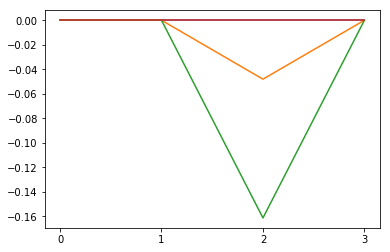
\includegraphics[width=\linewidth]{images/subst2/ef1_means_neg.png}
    \caption{}
  \end{subfigure}
  \begin{subfigure}[b]{0.3\linewidth}
    \includegraphics[width=\linewidth]{images/subst2/ef2_means_neg.png}
    \caption{}
  \end{subfigure}
  \caption{Mean Negative envy}
  \label{fig:efk}
  \small
    (a), (b), and (c) represent mean negative envy (envy) present in MNW allocations after dropping 0, 1, and 2 goods, respectively for additive utilities. (d), (e), (f), (g), (h), (i), (j), (k), and (l) represent that for complementing, substituting type-1, substituting type-2 utilities, respectively.
\end{figure}


Figure 5 plots mean envy between the agents after dropping 0, 1, and 2 goods for all MNW allocations. Mean envy-freeness raises with drops of 0, 1 and 2 goods as expected. The difference is greater from EF0 to EF1 than from EF1 to EF2 which is almost the same. This indicates when agents drop the first good in EF1 calculation, though it is known to drop the one which is valued the most by others, the first drop has a very high utility. Also noticeable is the decrease in envy-freeness with decrease in the number of goods. It is visible regardless of the type of utility or the number of goods being dropped. Figure 6 shows the mean positive envy (non-envy) in the allocation which closely follows and reflects the figure 5 mean envy plot.

Figure 7 plots the mean negative envy in the allocations after dropping 0, 1, and 2 goods for EF0, EF1, and EF2, respectively. Mean negative envy plot reflects association with Figure 4 - Percent EFk. It is the plot of envy values for the agents who negatively envies other agents. Similar to Figure 4, EF2 shows zero envy. The same high EF1 pattern as Figure 4 is visible in Figure 7 with some allocations showing zero negative envy.


% DFs additive
\begin{figure}[h!]
  \centering
  \begin{subfigure}[b]{0.47\linewidth}
    \includegraphics[width=\linewidth]{images/add/pdf_additive_10.png}
    \caption{}
  \end{subfigure}
  \begin{subfigure}[b]{0.47\linewidth}
    \includegraphics[width=\linewidth]{images/add/pdf_additive_8.png}
    \caption{}
  \end{subfigure}
  \begin{subfigure}[b]{0.47\linewidth}
    \includegraphics[width=\linewidth]{images/add/pdf_additive_6.png}
    \caption{}
  \end{subfigure}
  \begin{subfigure}[b]{0.47\linewidth}
    \includegraphics[width=\linewidth]{images/add/pdf_additive_4.png}
    \caption{}
  \end{subfigure}
  \caption{Envy distribution curve for Additive Utilities}
  \label{fig:efk}
  \small
    Envy distribution of the entire sample space with additive utilities after dropping 0, 1, and 2 goods for number of goods (a) $m = 10$, (b) $m = 8$, (c) $m = 6$, (d) $m = 4$
\end{figure}

% DFs complementing
\begin{figure}[h!]
  \centering
  \begin{subfigure}[b]{0.47\linewidth}
    \includegraphics[width=\linewidth]{images/compl/pdf_complementing_10.png}
    \caption{}
  \end{subfigure}
  \begin{subfigure}[b]{0.47\linewidth}
    \includegraphics[width=\linewidth]{images/compl/pdf_complementing_8.png}
    \caption{}
  \end{subfigure}
  \begin{subfigure}[b]{0.47\linewidth}
    \includegraphics[width=\linewidth]{images/compl/pdf_complementing_6.png}
    \caption{}
  \end{subfigure}
  \begin{subfigure}[b]{0.47\linewidth}
    \includegraphics[width=\linewidth]{images/compl/pdf_complementing_4.png}
    \caption{}
  \end{subfigure}
  \caption{Envy distribution curve for Complementing Utilities}
  \label{fig:efk}
  \small
    Envy distribution of the entire sample space with complementing utilities after dropping 0, 1, and 2 goods for number of goods (a) $m = 10$, (b) $m = 8$, (c) $m = 6$, (d) $m = 4$
\end{figure}

% DFs substituting type-1
\begin{figure}[h!]
  \centering
  \begin{subfigure}[b]{0.47\linewidth}
    \includegraphics[width=\linewidth]{images/subst1/pdf_subst1_10.png}
    \caption{}
  \end{subfigure}
  \begin{subfigure}[b]{0.47\linewidth}
    \includegraphics[width=\linewidth]{images/subst1/pdf_subst1_8.png}
    \caption{}
  \end{subfigure}
  \begin{subfigure}[b]{0.47\linewidth}
    \includegraphics[width=\linewidth]{images/subst1/pdf_subst1_6.png}
    \caption{}
  \end{subfigure}
  \begin{subfigure}[b]{0.47\linewidth}
    \includegraphics[width=\linewidth]{images/subst1/pdf_subst1_4.png}
    \caption{}
  \end{subfigure}
  \caption{Envy distribution curve for Substituting type 1 Utilities}
  \label{fig:efk}
  \small
    Envy distribution of the entire sample space with substituting utilities type 1 after dropping 0, 1, and 2 goods for number of goods (a) $m = 10$, (b) $m = 8$, (c) $m = 6$, (d) $m = 4$
\end{figure}

% DFs substituting type-2
\begin{figure}[h!]
  \centering
  \begin{subfigure}[b]{0.47\linewidth}
    \includegraphics[width=\linewidth]{images/subst2/pdf_subst2_10.png}
    \caption{}
  \end{subfigure}
  \begin{subfigure}[b]{0.47\linewidth}
    \includegraphics[width=\linewidth]{images/subst2/pdf_subst2_8.png}
    \caption{}
  \end{subfigure}
  \begin{subfigure}[b]{0.47\linewidth}
    \includegraphics[width=\linewidth]{images/subst2/pdf_subst2_6.png}
    \caption{}
  \end{subfigure}
  \begin{subfigure}[b]{0.47\linewidth}
    \includegraphics[width=\linewidth]{images/subst2/pdf_subst2_4.png}
    \caption{}
  \end{subfigure}
  \caption{Envy distribution curve for Substituting type 2 Utilities}
  \label{fig:efk}
  \small
    Envy distribution of the entire sample space with substituting utilities type 2 after dropping 0, 1, and 2 goods for number of goods (a) $m = 10$, (b) $m = 8$, (c) $m = 6$, (d) $m = 4$
\end{figure}


Figure 8-11 plot the distributions of envy for simulated 1000 samples. As discussed about other plots, the decrease in number of goods can directly be seen in increase in number of envied allocations. These curves give a nice shape to the envy calculations before and after dropping goods for EF0, EF1, and EF2 calculations. Figure 8-11 show both, final envy after dropping the good and that sorted on the sampling x-axis which forms a smooth shape with rest of the distribution curve.

\section{MNW and EFk}
In this section, we analyze the relation between maximum Nash welfare and envy-freeness up to k goods.

We already know MNW allocations for additive utility values are envy-free up to one good (EF1) \cite{caragiannis2016unreasonable}. The experiments on goods with additive utilities in previous section provide the experimental evidence to that fact.

In previous section, we conduct experiments on complementary and substitute goods. We have simulated the complements and substitutes of the goods in the market in terms of the dependency of utility valuation for pairs of goods. An interesting fact emerge from the plots is that, all of the MNW allocations are envy-freeness up to 2 goods.

We classify the complementary and substitute valuations as dependent goods.

\textit{Definition 5.1} Dependent good valuations.
Dependent good is the good $x$ who's value for an agent $V(x)$ depends on whether the agent gets some other set of goods $Y$ in allocation $\mathcal{A}$ or not.

Extending the idea of EF1 of additive goods, in this section, we formally affirm the envy-freeness up to k goods (EFk) for dependent goods.

\subsubsection{Theorem} \textit{Every MNW allocation is envy free up to k goods (EFk) for dependent valueations over indivisible goods where the valuations of an agent for goods show dependency on k other goods.}

\textit{Proof} $\mathcal{A}$ is a MNW allocation for n agents. 


\hrule
x
\hrule

\subsubsection{Definition 3} Network Embedding

For a graph G, a network embedding is a ming function $\phi : V \mapsto \mathbb{R}^{|V|xd}$ where $d << |V|$. Mapping $\phi$ defines the latent representation embedding vector space for each node $v \in V$. $\phi(v)$ denotes the embedding vector for $v$.

\subsubsection{Problem 1} Influence embedding \cite{zhang2013social}

Social influence locality models the probability of $v$'s action conditioned on its neighboring network $G^n_v$ where n is the depth of neighbor to monitor. So, given $G_v^n$ and $S_v^t = \{s^t_v : v \in \Gamma_v^n / \{v\} \}$
Our input to the problem is N instances of 3-tuple $(v, a, t)$ where $v$ is the node, $a$ is the action, and $t$ is the timestamp of the action.


\subsection{Inflowalk}

Our method is highly inspired by the DeepWalk \cite{perozzi2014deepwalk} random walk method described in the preliminaries. It consists of three simple steps. First, creating a network embedding based only on the network structure. Second, creating the network embedding based on the influence network. Third, concatenation and merging of the embeddings.

\subsubsection{Node Embedding}

The random walk generator takes graph G  and samples uniformly a random vertex $v_i$ as the start of the random walk. Then it samples another random node from neighbors to create the next node of the path. It keeps on repeating this till we get a path length of the max size defined as an input to the program.

Next step is to take each of the generated path one by one and pass it to the skip-gram \cite{mikolov2013efficient} Word2Vec model. The word2vec receives each paths one by one like a sentence and updates node embedding for each node in the path and further the graph.

\subsubsection{Influence Embedding}

The influence embedding layer is very similar to the node embedding layer in the sense that it receives paths, pass it to word2vec skip-gram model and generate the embeddings. The difference is instead of random sampling, this time we sample the neighbor for the choice of path based on current nodes influence on the neighbor. The influence here is defined as a normalized vector of the amount of interaction between the noes.

\subsubsection{Concatenation Layer}

Concatenation layer takes as input the two same N sized embeddings and output a concatenated version of the embeddings for each node. It's a simple fully connected layer with 2N inputs and N outputs to represent N dimensional embedding.

\section{Experiments}

\subsection{Datasets}

We use three real-world datasets for our experiments - Digg \cite{hogg2012social}, Twitter \cite{de2013anatomy}, Citeseer \cite{chung1997spectral}. We have reduced the size of the original datasets as per the available computational capability. Following table provides the details of the full datasets:

\begin{table}
  \caption{Dataset statistics}
  \begin{tabular}{ccc}
    \toprule
    Dataset&|V|&|E|\\
    \midrule
    Digg & 279,630 & 41,548,126 \\
    Twitter & 456,626 & 12,508,413 \\
    Citeseer & 3312 & 4732 \\
  \bottomrule
\end{tabular}
\end{table}

\subsection{Baselines}


\subsection{Experimental Parameter}

We set the window size of 20 for the walks of size 35 and we generate 80 walks (or less for influence network) for each path. Our final embedding size for each step is set to 128. We run 8 computation threads to speed up the embedding process.

\subsection{Results}

Table shows the result of the classification tasks performed on the three datasets using the two embeddings

\begin{table}
  \caption{Model Classification Accuracy}
  \begin{tabular}{cccc}
    \toprule
    Model&Digg&Twitter&Citeseer\\
    \midrule
    DeepWalk&0&0&0\\
    InfloWalk&0&0&0\\
  \bottomrule
\end{tabular}
\end{table}


\section{Conclusion and Future Work}
Most of the existing node embedding research focus on static graphs where one node doesn't usually affect any other node. This approach doesn't make use of the information available in the interaction between the nodes. InfloWalk successfully captures the interaction between nodes and produces embedding which reflects the same. This specifically helps in the tasks like node classification where instead of just the node connections, if the node interaction is used, we should get better spatial distribution of nodes in the embedded vector space. This is evident from the experiments we conducted on three real-world dataset.

Currently, the node embeddings are being trained separately. In the future, we'll like to work on a model that combines uses this information along with user features such as geolocation, text content features (tweet vectors, LIWC) to produce a more grounded embedding. Features such as language, emotions, etc. may probably be a better indicator of the influence

\begin{acks}
I would like to acknowledge the class of CS 584 - Advanced Data Mining, Fall'18 for the introduction to all the interesting concepts in data mining which further became part of this paper. I would also like to thank Prof. Philip S. Yu and Chenwei Zhang for an interesting course
\end{acks}


\bibliographystyle{ACM-Reference-Format}
\bibliography{sample-bibliography}

\end{document}
